\documentclass{scrbook}

% Language setting
% Replace `english' with e.g. `spanish' to change the document language
\usepackage[english]{babel}

% Set page size and margins
% Replace `letterpaper' with `a4paper' for UK/EU standard size
\usepackage[a4paper,top=2cm,bottom=2cm,left=3cm,right=3cm,marginparwidth=1.75cm]{geometry}

\setkomafont{author}{\scshape}
\usepackage{blindtext}

% Useful packages
\usepackage{amsmath}
\usepackage{graphicx}
\usepackage[colorlinks=true, allcolors=blue]{hyperref}

\usepackage{layouts}

\usepackage{caption}
\usepackage{subcaption}

\title{Optimal Vehicle Maneuvers}
\author{Arvind Balachandran\thanks{I never procrastinate}}
\subtitle{Not a course in vehicle dynamics, of course!}
\subject{Technical Report}

\usepackage{xspace}
\newcommand{\uvec}[1]{\textit{$\textit{u}_{\textit{#1}}$}\xspace}
\newcommand{\tsim}{\textit{$\textit{t}$}\xspace}
\newcommand{\mass}{\textit{$\textit{m}$}\xspace}

\usepackage{matlab-prettifier}

\begin{document}
\maketitle

\chapter[Particle model optimization]{Friction-limited particle with and without rate-limitation}
Investigating the friction-limited particle and the friction-limited particle with rate-limited direction control with a comparison. 

The optimization problems follow the following general equation structure: 
\begin{align}
    & \underset{u}{\text{Min}}
    & & J\\
%
    & \text{subject to} 
    & & f_u(u) <= 0\\
%
    &&& f_o(x,u) <= 0 \\
%
    &&& \dot x = f(x,u),\\
%
    &&& x_0,\ x_f,
\end{align}
where $u$ is(are) the optimization variable(s), $J$ is the cost function, $f_u(u) <= 0$ and $f_o(x,u) <= 0$ denote the constraints on the $u$ and the states $x$, $\dot x = f(x,u)$ are the ODEs or dynamic constraints, and $x_0,\ \&\ x_f$ are the boundry conditions. 

\begin{description}
    \item[Opimization variables:] the longitudinal and lateral forces $u_x$ and $u_y$ on the vehicle. 
    \item[Cost function:] to minimize time $t$.
    \item[Constraints:] The forces on the vehicle are limited elliptically, i.e., \begin{equation*}
        u_x^2 + u_y^2 \leq (\mu m g)^2.
    \end{equation*}
    The force limit on the vehicle for the rate-limited direction control is given by \begin{align*}
        u_1^2 \leq (\mu m g)^2.
    \end{align*}\par The obstacle is given by the following equation:
    \begin{align*}
        \left(\frac{x - X_a}{R_1}\right)^n + \left(\frac{y}{R_2}\right)^n \geq 1
    \end{align*}
    \item[Vehicle model:] The friction-limited particle is given as follows: \begin{align*}
        \dot x &= v_x, \\
        \dot x &= v_x, \\
        m\,\dot v_x &= u_x,\\
        m\,\dot v_x &= u_y. \\
    \end{align*}
    The friction-limited particle with rate-limited direction control is given as follows: \begin{align*}
        \dot x &= v_x, \\
        \dot x &= v_x, \\
        m\,\dot v_x &= u_1\,\cos\left(\delta\right),\\
        m\,\dot v_y &= u_1\,\sin\left(\delta\right), \\
        \dot \delta &= u_2. \\
    \end{align*}
    \item[Miscellaneous constraints:] In order to ensure that the solution is within the desired operating space, certain miscellaneous constraints are included such as, \begin{align*}
        x_0 \leq x \leq x_f\\
        y_0 \leq y \leq y_f\\
        y_{min} \leq y \leq y_{max} \\
        0 \leq v_x 
    \end{align*} 
    For the rate-limited direction control model, the steering angle and steering rate is also constrained, i.e., \begin{align*}
        |\delta| \leq \delta_{max}, \\
        |\dot\delta| \leq \dot\delta_{max}, \\
    \end{align*}
\end{description}

The model, optimization, and obstacle parameters are presented in Tables~\ref{tab:flp_mdlparams},~\ref{sub@tab:flp_optparams}, and~\ref{sub@tab:flp_obsparams}, respectively. 

\begin{table}[h!]
    \begin{subtable}[h]{0.3\textwidth}
        \centering
        \begin{tabular}{c|c}
            - & value \\
            \hline
            $m$ & 500\,kg\\
            $g$ & 9.8\,m/s\textsuperscript{2}\\
            $\mu$ & 0.8\\
        \end{tabular}
        \caption{Model parameters}
        \label{tab:flp_mdlparams}
    \end{subtable}
    \hfill
    \begin{subtable}[h]{0.3\textwidth}
        \centering
        \begin{tabular}{c|c}
            - & value \\
            \hline
            $x_0$ & 0\,m\\
            $x_f$ & 100\,m\\
            $y_0$ \& $y_f$ & 1\,m\\
            $v_x$ & 40\,km/h\\
            $v_y$ & 0\,km/h
        \end{tabular}
        \caption{Initial parameters}
        \label{tab:flp_optparams}
    \end{subtable}
    \hfill
    \begin{subtable}[h]{0.3\textwidth}
        \centering
        \begin{tabular}{c|c}
            - & value \\
            \hline
            $X_a$ & 50\,m\\
            $R_1$ & 2\,m\\
            $R_2$ & 1.5\,m\\
            $n$ & 6\\
        \end{tabular}
        \caption{Obstacle parameters}
        \label{tab:flp_obsparams}
    \end{subtable}
    \caption{Model, optimization, and obstacle parameters.}
    \label{tab:temps}
\end{table}

The optimal control problem (OCP), was solved with direct multiple-shooting with 40 control intervals for the optimization using Matlab and CasADi. The ODE was solved using the fixed-step Runge-Kutta 4 integration method. 

The results of the optimization are presented in 

\begin{figure}[h!]
    \centering
    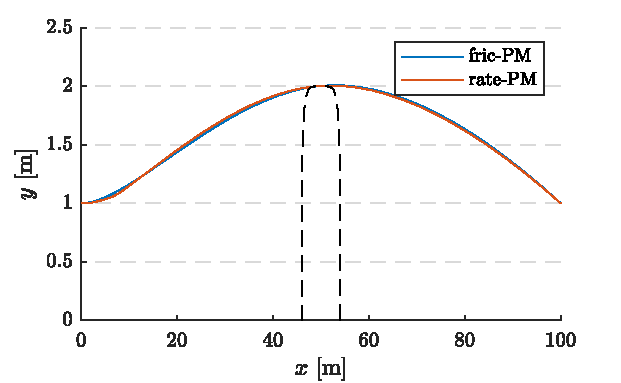
\includegraphics{figures/flp_avoid.pdf}
    \caption{Obstacle avoidance trajectory for the friction- and rate-limited particle model.}
    \label{fig:res_traj_p1}
\end{figure}

\pagebreak

\begin{table}[h]
    \centering
    \begin{tabular}{c|c|c}
        - & min $t$ & min $-v_f$ \\
        \hline
        $t$ & 3.83\,s & 3.94\,s \\
        $v_x(t_f)$ & 147.59\,km/h & 146.03\,km/h\\
    \end{tabular}
    \caption{Results for friction-limited and rate-limited particle model.}
    \label{tab:prob1_res}
\end{table}

From Table~\ref{tab:prob1_res}, it is clear that the friction-limited particle model (fric-PM) is slightly faster than the rate-limited particle model (rate-PM). 
This is because in rate-PM the rate of change of direction of the particle is limited and as a result, the ability of the vehicle to make a sharp turn is restricted and thus takes a longer time to complete the maneuver. 
This is visible in the control signals and state variables for the optimal trajectory shown in Figure~\ref{fig:prob1_res_detail}. 

Additional constraints and initial values for the firc-PM and rate-PM are presented in Table~\ref{tab:const_p1}. 

\begin{table}[h]
    \centering
    \begin{subtable}[h]{0.4\textwidth}
        \begin{tabular}{c|c||c|c}
            \multicolumn{2}{c||}{fric-PM} & \multicolumn{2}{c}{rate-PM}\\
            \hline
            $y_{max}$ & 5 & $\delta_{max}$ & $\pi/2$ \\
            - & - & $\dot\delta_{max}$ & $\pi/6$ 
        \end{tabular}
        \caption{Constraints.}
        \label{tab:const_p1a}
    \end{subtable}
    % \hfill
    \begin{subtable}[h]{0.4\textwidth}
        \begin{tabular}{c|c||c|c}
            \multicolumn{2}{c||}{fric-PM} & \multicolumn{2}{c}{rate-PM}\\
            \hline
            $v_x$ & 40\,km/h & $v_x$ & 40\,km/h
        \end{tabular}
        \caption{Initial conditions.}
        \label{tab:const_p1a}
    \end{subtable}
    \caption{Constraints for the fric-PM and rate-PM.}
    \label{tab:const_p1}
\end{table}

\begin{figure}[h!]
    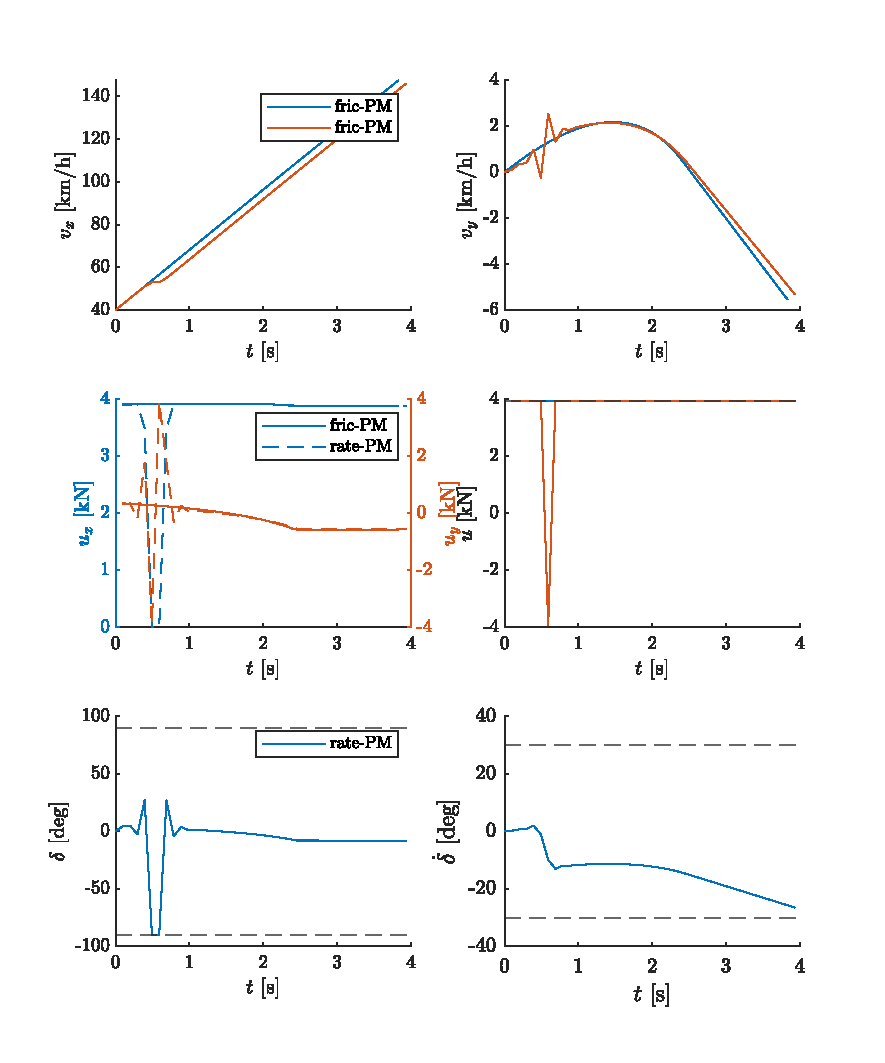
\includegraphics{figures/flp_avoid_detailed.pdf}
    \caption{Detailed optimal trajectory states and control inputs for friction- and rate-limited particle models.}
    \label{fig:prob1_res_detail}
\end{figure}

\noindent\fbox{%
    \parbox{\textwidth}{%
        \textbf{Some reflections}: \newline
        The fric-PM can converge faster than the rate-PM in some cases. 
        Since 'ipopt' is used to solve the optimization problem, fric-PM is more sensitive toward the initializations (initial guesses). 
        Therefore, additional constraints may be necessary to improve convergence.
        Furthermore, the rate-PM does not have this problem and thus can have a lower computational time.
        However, the computational time can get long with 'bad' initialization conditions. 
        The convergence of this model seems better than the fric-PM.
        
        It is worth mentioning that the terms 'improved convergence' and 'better convergence' mean the ability of the solver to produce an 'optimal solution found' even with ridiculous guesses. However, one should take care not to fall into local minima pits. 
    }%
}

\section{Code}
The source code for this problem can be found at \newline \href{https://github.com/arvba41/optimal_vehicle_maneuvers/tree/main/uppgift/ugf1}{https://github.com/arvba41/optimal\_vehicle\_maneuvers}.
\chapter[Double-Track Maneuver Optimization]{Maneuver with DT for hairpin 4\textsuperscript{th} degree super ellipse, without LT or WT.}

In addition to the double-track (DT) model equations state equations,
% \begin{align*}
%     \dot X_p &= v_x\,\cos(\psi) - v_y\,\sin(\psi),\\
%     \dot Y_p &= v_x\,\sin(\psi) + v_y\,\cos(\psi),\\
%     \dot \psi &= r,\\
%     \dot v_x &= \frac{F_x}{m} + v_y\,r,\\
%     \dot v_Y &= \frac{F_Y}{m} + v_x\,r,\\
%     \dot r &= \frac{M_z}{I_{zz}}.
% \end{align*}
the input forces are filtered using a low pass filter with a time constant $\tau_f$ to prevent NaN errors during the optimization.
\begin{align}
    \dot F_{x(f)} &= \frac{1}{\tau_f}\,\left(F_{x(f)}^* - F_{x(f)}\right),\\
    \dot F_{x(r)} &= \frac{1}{\tau_f}\,\left(F_{x(r)}^* - F_{x(r)}\right),
\end{align}
where $F_{x(f)}^*$ and $F_{x(r)}^*$ are the inputs to the model.

The hairpin is modeled as two ellipses,
\begin{align}
    \frac{x}{R_1^i} + \frac{y}{R_2^i} & \geq 1, & \frac{x}{R_1^o} + \frac{y}{R_2^o} & \leq 1.
    % \frac{x}{R_1^î} + \frac{y}{R_2^i} &\geq 1 \ \text{Inner ellipse},
    % \frac{x}{R_1^o} + \frac{y}{R_2^o} &\leq 1 \ \text{outer ellipse}.
\end{align}
A straightforward model of combined forces is based on the friction ellipses and the Magic Formula. The tire parameters are taken from Berntorp, Karl, et al. "Models and methodology for optimal trajectory generation in safety-critical road–vehicle manoeuvres." Vehicle System Dynamics 52.10 (2014): 1304-1332.

The nominal normal force $F_z$ resting on the respective wheel in the steady state is given by
\begin{align}
    F_{z(1)} &= \frac{1}{2}\,mg\frac{l_r}{l_f+l_r}, & F_{z(2)} &= \frac{1}{2}\,mg\frac{l_r}{l_f+l_r}, & F_{z(3)} &= \frac{1}{2}\,mg\frac{l_f}{l_f+l_r}, & F_{z(4)} &= \frac{1}{2}\,mg\frac{l_f}{l_f+l_r}.
\end{align}

\section{Constrains}
\begin{description}
    \item[$v_x > 0$] to avoid $\div$ by zero error while calculating the lateral slips, $\alpha$.
    \item[$-\delta_{max} \leq \delta \leq \delta_{max}$] steering angle limit.
    \item[$-\dot\delta_{max} \leq \dot\delta \leq \dot\delta_{max}$] steering angle rate limit.
    \item[$-\epsilon\,D_{x(f)} \leq F_{x(f)}^* \leq \epsilon\,D_{x(f)}$], limiting the forces on the front wheel, and $\epsilon$ is a number close to 1 to avoid NaN errors. 
    \item[$-\epsilon\,D_{x(r)} \leq F_{x(r)}^* \leq 0$], limiting the forces on the rear wheel.
    \item[$X_f - \beta \leq X_p(\text{end}) \leq X_f + \beta $], Allowing some error on the final $X_P$.
    \item[$Y_f - \beta \leq Y_p(\text{end}) \leq Y_f + \beta $], Allowing some error on the final $Y_P$.
\end{description}
The model is front-wheel driven but can brake on all four wheels.

\section{Cost function}
The const function $J$ is defined as 
\begin{align}
    J &= \min{\left(t + 0.5\beta\right)},
\end{align}
The number 0.5 is arbitrarily chosen. 

The vehicle parameters and constraints for the the optimal control problem are presented in Table \ref{tab:ocp_prob2}.

\begin{table}[h!]
    \begin{subtable}{0.3\textwidth}
        \begin{tabular}{c|c}
            parameter & value\\
            \hline
            $m$ & 2100\,kg\\
            $l_f$ & 1.3\,m \\     
            $l_r$ & s1.5\,m \\
            $w$ & 0.8\,m\\
            $g$ & 9.82\,m/s\textsuperscript{2}\\
            $I_{zz}$ & 3900\,kgm\textsuperscript{2}\\
        \end{tabular}
        \caption{Vehicle parameters}
    \end{subtable}
    \hfill
    \begin{subtable}{0.3\textwidth}
        \begin{tabular}{c|c}
            parameter & value\\
            \hline
            $R_1^i$ & 2\,m \\
            $R_2^i$ & 50\,m \\
            $R_1^o$ & 7\,m \\
            $R_2^o$ & 55\,m \\
        \end{tabular}
        \caption{Hairpin parameters}
    \end{subtable}
    \hfill
    \begin{subtable}{0.3\textwidth}
        \begin{tabular}{c|c}
            parameter & value\\
            \hline
            $\delta_{max}$ & 30$^\circ$ \\
            $\dot\delta_{max}$ & 45$^\circ$/s \\
            $\tau_f$ & 0.1\,s\\
            $\epsilon$ & 0.99\\
        \end{tabular}
        \caption{Constrains}
    \end{subtable}
    \caption{The vehicle, hairpin, and constraints for the DT-optimal vehicle Maneuver problem.}
    \label{tab:ocp_prob2}
\end{table}

The optimal trajectory for the DT model through the hairpin is presented in Figure~\ref{fig:DT_hairpin_path}. 

\begin{figure}[h!]
    \centering
    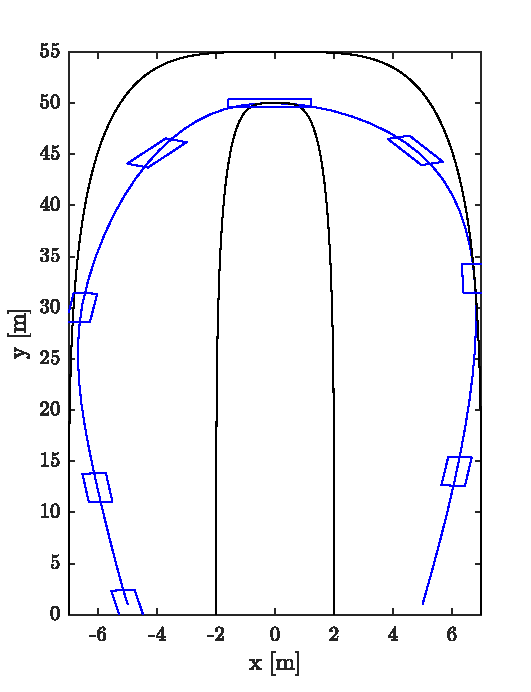
\includegraphics{figures/prob2_DT_path.pdf}
    \caption{Optimal trajectory for a harpin maneuver with minimum time for DT-model.}
    \label{fig:DT_hairpin_path}
\end{figure}

The states and forces acting on the wheels for the DT model for the hairpin are presented in Figure~\ref{fig:DT_hairpin_path_detail}. 

\begin{figure}[p]
    \centering
    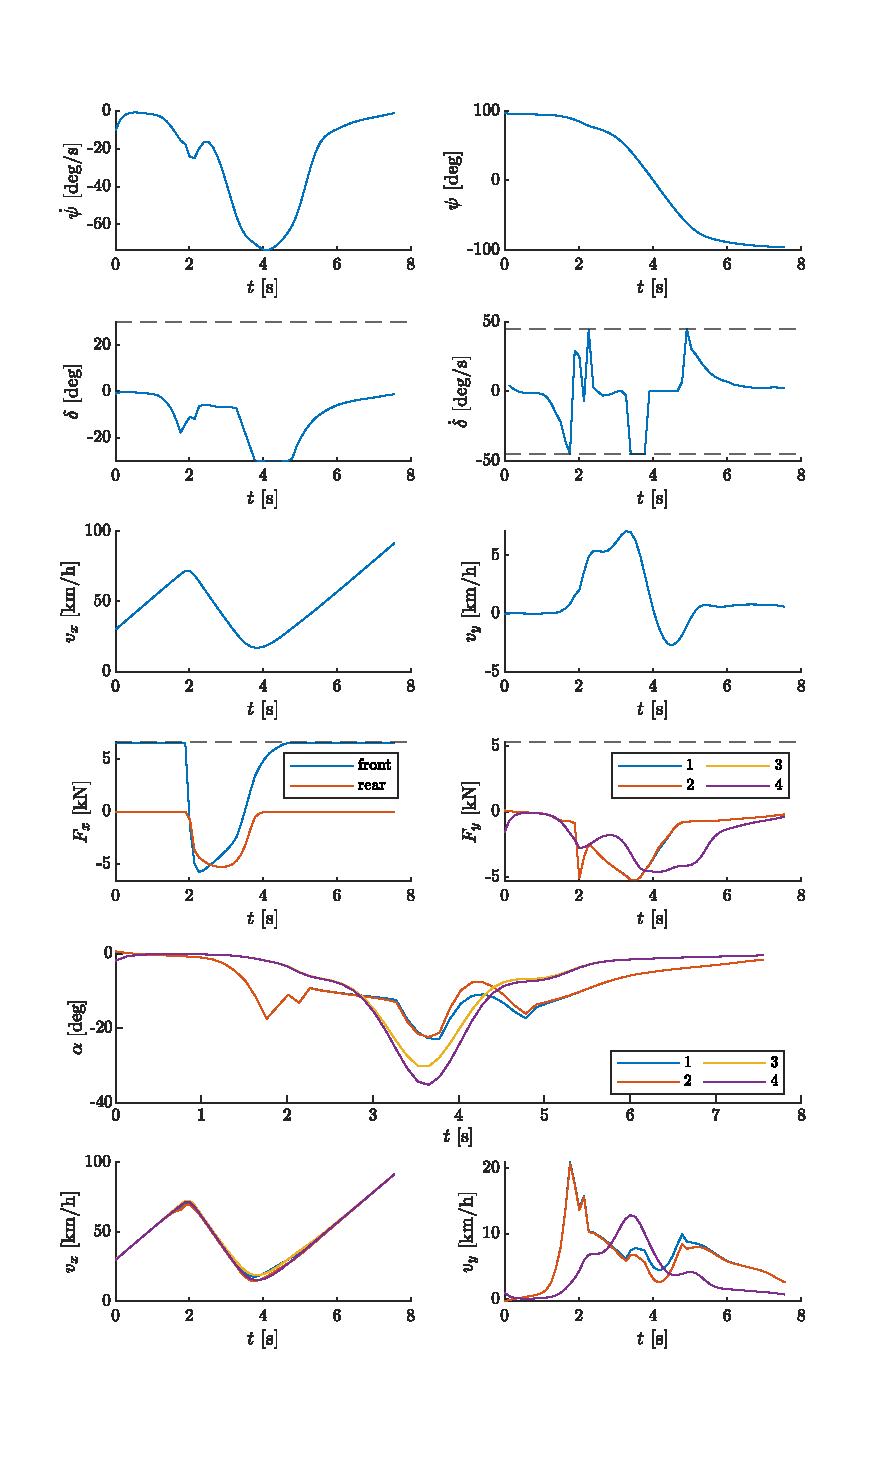
\includegraphics{figures/prob2_DT_path_detail.pdf}
    \caption{velocities, forces, and steering angels during the optimal trajectory for a harpin maneuver with minimum time for DT-model.}
    \label{fig:DT_hairpin_path_detail}
\end{figure}


\noindent\fbox{%
    \parbox{\textwidth}{%
        \textbf{Some reflections}: \newline
        The OCP for the DT model hairpin turn maneuver can have difficulty finding the optimal solution if the initial guesses are non-trivial. Therefore to improve convergence, the height of the hairpin was slowly increased, and the simulation results from the previous iterations were used as initializations for the next.
    }%
}

\section{Code}

The source code for this problem can be found at \newline \href{https://github.com/arvba41/optimal_vehicle_maneuvers/tree/main/uppgift/ugf2}{https://github.com/arvba41/optimal\_vehicle\_maneuvers}.

% $\mathbf{v_x > 0}$, to avoid $\div$ by zero error while calculating the lateral slips, $\alpha$.\\
% $\mathbf{-\delta_{max} \leq \delta \leq \delta_{max}}$, steering angle limit.\\
% $\mathbf{-\dot\delta_{max} \leq \dot\delta \leq \dot\delta_{max}}$, steering angle limit.\\
% opti.subject_to(-deltamax<=delta<=deltamax);    % steering angle limit
% opti.subject_to(-ddeltamax<=ddelta<=ddeltamax); % steering rate limit


\chapter{Verification of brake or evade criteria}

To verify the brake or evade criteria the following OCP was formulated:
\begin{align}
    & \underset{u}{\text{Min}}
    & & \mu\\
%
    & \text{subject to} 
    & & f_u(u) <= 0\\
%
    &&& \dot x = f(x,u),\\
%
    &&& x_0,\ x_f.
\end{align}

\section{Straight-line braking}
For straight-line braking, the following constraints are set up:
\begin{align}
    f_u(u): && 0 \geq F_x &\leq -F_{\text{max}} & F_y &= 0,\\
    \dot x = f(x,u): && \dot x &= v_x, & \dot y &= v_y, & \dot v_x &= \frac{F_x}{m}, & \dot v_y &= \frac{F_y}{m},\\
    x_0,\ x_f: && x(t_o) &= 0, & y(t_o) &= 0, & v_x(t_o) &= v_o, & v_y(t_o) &= 0,\\
    && x(t_f) &= x_f, & y(t_f) &= 0, & v_x(t_f) &= 0, & v_y(t_f) &= 0,
\end{align}
where $F_{\text{max}} = \mu m g$. The parameters of the vehicle are presented in Table~\ref{tab:brake_evade_params}.

The numerical verification for the break or evade criteria for straight-line braking is presented in Table~\ref{tab:brake_evade_straight_line_braking}.

\begin{table}[h!]
    \begin{subtable}{0.4\textwidth}
        \begin{tabular}{c|c}
            Parameters & Value \\
            \hline
            $m$ & 2000\,kg \\
            $g$ & 9.81\,m/s\textsuperscript{2} \\
        \end{tabular}
        \caption{Vehicle PM parameters.}
        \label{tab:brake_evade_params}
    \end{subtable}
    \hfill
    \begin{subtable}{0.6\textwidth}
        \begin{tabular}{c|c|c|c}
            & & Analytical & Simulation\\
            & $x_f$ & $\mu$ & $\mu$ \\
            % [m] & [-] & [m] & [-] \\
            \hline
            Dry Asphalt & 20.3\,m & 1 & 1.0043\\
            Wet Asphalt & 34\,m & 0.6 & 0.5996\\
            Ice Asphalt & 68\,m & 0.3 & 0.2998\\
        \end{tabular}
        \caption{Numerical and analytical solutions for road friction for straight-line braking with $v_0 = 20$\,m/s.}
        \label{tab:brake_evade_straight_line_braking}
    \end{subtable}
    \caption{Brake or evade for straight-line braking.} 
    \label{tab:brake_evade_straight}
\end{table}

\subsection{Code}
The source code for this problem can be found at \newline \href{https://github.com/arvba41/optimal_vehicle_maneuvers/blob/main/uppgift/ugf3/brake_or_evade_p1.m}{https://github.com/arvba41/optimal\_vehicle\_maneuvers}.

\section{Evading}
This section presents the numerical verification of evading criteria considering a PM.

\subsection{Wet asphalt maximum obstacle height}
To verify the largest obstacle that can be avoided without any braking on wet asphalt,the following OCP is formulated:
\begin{align}
    & \underset{u}{\text{Max}}
    & & & y(t_f)\\
%
    & \text{subject to} 
    & & & F_x &= 0 &0 \leq F_y &\leq F_{\text{max}},\\
%
    &&& & \dot x &= v_x, & \dot y &= v_y, & \dot v_x &= \frac{F_x}{m}, & \dot v_y &= \frac{F_y}{m},\\
%
    &&& & x(t_o) &= 0, & y(t_o) &= 0, & v_x(t_o) &= v_o, & v_y(t_o) &= 0,\\
    &&& & x(t_f) &= x_f,
\end{align}
where $F_{\text{max}} = \mu m g$, and the vehicle parameters are presented in Table~\ref{tab:brake_evade_params}.
\begin{table}[h!]
    \centering
    \begin{tabular}{c|c|c|c|c}
        & & & Analytical & Simulation\\
        $x_f$ & $v_0$ & $\mu$ & $y(t_f)$ & $y(t_f)$ \\
        % [m] & [-] & [m] & [-] \\
        \hline
        34\,m & 20\,m/s & 0.6 & 8.5\,m & 8.5053\,m \\
    \end{tabular}
    \caption{Numerical and analytical solutions for maximum obstacle height that a vehicle can avoid.}
\end{table}
\subsubsection{Code}
The source code for this problem can be found at \newline \href{https://github.com/arvba41/optimal_vehicle_maneuvers/blob/main/uppgift/ugf3/brake_or_evade_p2a.m}{https://github.com/arvba41/optimal\_vehicle\_maneuvers}.
\subsection{Minimum required friction}
To verify the minimum required friction to avoid an obstacle with a height of 1.7\,m at a distance of 34\,m, the following optimization problem was formulated:
\begin{align}
    & \underset{u}{\text{Min}}
    & & & \mu\\
%
    & \text{subject to} 
    & & & F_x &= 0 &0 \leq F_y &\leq F_{\text{max}},\\
%
    &&& & \dot x &= v_x, & \dot y &= v_y, & \dot v_x &= \frac{F_x}{m}, & \dot v_y &= \frac{F_y}{m},\\
%
    &&& & x(t_o) &= 0, & y(t_o) &= 0, & v_x(t_o) &= v_o, & v_y(t_o) &= 0,\\
    &&& & x(t_f) &= x_f, & y(t_f) &= y_f,
\end{align}
where $F_{\text{max}} = \mu m g$, and the vehicle parameters are presented in Table~\ref{tab:brake_evade_params}.
\begin{table}[h!]
    \centering
    \begin{tabular}{c|c|c|c|c}
        & & & Analytical & Simulation\\
        $x_f$ & $y_f$ & $v_0$ & $y(t_f)$ & $y(t_f)$ \\
        % [m] & [-] & [m] & [-] \\
        \hline
        34\,m & 1.7\,m & 20\,m/s & 0.12 & 0.1199 \\
    \end{tabular}
    \caption{Numerical and analytical solutions for the minimum required friction to avoid an obstacle.}
\end{table}
\subsubsection{Code}
The source code for this problem can be found at \newline \href{https://github.com/arvba41/optimal_vehicle_maneuvers/blob/main/uppgift/ugf3/brake_or_evade_p2b.m}{https://github.com/arvba41/optimal\_vehicle\_maneuvers}.
\subsection{Minimum distance to object}
To verify the minimum distance to an object with a height of 1.7\,m on wet asphalt, the following optimization problem was formulated:
\begin{align}
    & \underset{u}{\text{Max}}
    & & & x(t_f)\\
%
    & \text{subject to} 
    & & & F_x &= 0 &0 \leq F_y &\leq F_{\text{max}},\\
%
    &&& & \dot x &= v_x, & \dot y &= v_y, & \dot v_x &= \frac{F_x}{m}, & \dot v_y &= \frac{F_y}{m},\\
%
    &&& & x(t_o) &= 0, & y(t_o) &= 0, & v_x(t_o) &= v_o, & v_y(t_o) &= 0,\\
    &&& & y(t_f) &= y_f,
\end{align}
where $F_{\text{max}} = \mu m g$, and the vehicle parameters are presented in Table~\ref{tab:brake_evade_params}.
\begin{table}[h!]
    \centering
    \begin{tabular}{c|c|c|c|c}
        & & & Analytical & Simulation\\
        $\mu$ & $y_f$ & $v_0$ & $x(t_f)$ & $x(t_f)$ \\
        % [m] & [-] & [m] & [-] \\
        \hline
        0.6 & 1.7\,m & 20\,m/s & 15.2\,m & 15.2006\,m\\
    \end{tabular}
    \caption{Numerical and analytical solutions for the maximum distance to an obstacle that can be avoided.}
\end{table}
\subsubsection{Code}
The source code for this problem can be found at \newline \href{https://github.com/arvba41/optimal_vehicle_maneuvers/blob/main/uppgift/ugf3/brake_or_evade_p2c.m}{https://github.com/arvba41/optimal\_vehicle\_maneuvers}.

\pagebreak
The width of a column is:
\printinunitsof{mm}\prntlen{\textwidth} (\printinunitsof{in}\prntlen{\textwidth}) \\
The height of a column is:
\printinunitsof{mm}\prntlen{\textheight} (\printinunitsof{in}\prntlen{\textheight}) \\



\end{document}